\documentclass{article}

\usepackage[utf8]{inputenc}
\usepackage[backend=biber, style=numeric]{biblatex}
\usepackage[dutch]{babel}
\usepackage{fancyhdr}
\usepackage{graphicx}
\usepackage{float}
\usepackage{booktabs}
\usepackage{subcaption}


\pagestyle{fancy}
\fancyhf{}
\rhead{ Scaling }
\lhead{Meetrapport}
\rfoot{Pagina \thepage }

\begin{document}
\author{Dimitry Volker}
\makeatletter
    \begin{titlepage}
        \begin{center}
            {\huge \bfseries  \@title }\\[2ex] 
            {\LARGE Meetrapport, Snelheid - Scaling}\\[10ex]
            
            {\large \@author - 1661152}\\
            {\large Jasper van Hulst - 1660498}\\[5ex]
            {\large \@date}
            
            \vskip4em%
        \end{center}
    \end{titlepage}
\makeatother
\thispagestyle{empty}

\clearpage

\renewcommand{\contentsname}{Inhoudsopgave}
\tableofcontents

\clearpage

\section{Doel}
Het schalen van een afbeelding is op diverse manieren voor elkaar te krijgen. Er bestaan 3 algoritmes die veel op elkaar lijken "Nearest-neighbour Interpolation", "Bilinear Interpolation" en "Bicubic Interpolation". Echter willen we weten welk algoritme het beste werkt samen met de gezichtsherkenning, aangeleverd door Arno.  

\begin{center}
    "Welk algoritme integreert het beste met de gezichtsherkenning algoritme van Arno?".   
\end{center}

\section{Hypothese}

Het lijkt ons aannemelijk dat "Bicubic Interpolatie" het beste zal functioneren. Door een groter veld te pakken (16 bij 16 pixels) zullen de overgangen zachter zijn en blijven details meer intact.

\section{Onderzoeksmethode}
Om te kijken wat het beste integreert met de gezichtsherkenning, schalen we zelf onze afbeelding en laten we het algoritme van gezichtsherkenning erop los. Dit doen we met twee schalingsfactoren:

\begin{itemize}
    \item 0.75;
    \item 1.25;
\end{itemize}

\begin{figure}[H]
    \centering
    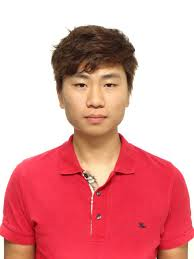
\includegraphics{assets/male-1.png}
    \caption{Orginele afbeelding}
    \label{fig:my_label}
\end{figure}

\section{Resultaten}

\subsection{Schalingsfactor 0.75}

\begin{figure}[H]
\centering
    \begin{subfigure}{.5\textwidth}
      \centering
      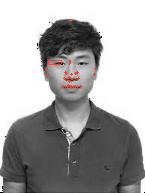
\includegraphics[]{assets/Bicubic_male_075.png}
      \caption{Bicubic, scalingfactor: 0.5}
      \label{fig:sub1}
    \end{subfigure}%
    \begin{subfigure}{.5\textwidth}
      \centering
      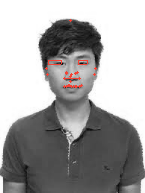
\includegraphics[]{assets/Bilinear_male_075.png}
      \caption{Bilinear, scalingfactor: 0.5}
      \label{fig:sub2}
    \end{subfigure}
    \begin{subfigure}{.5\textwidth}
      \centering
      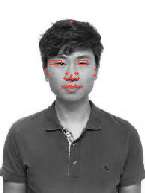
\includegraphics[]{assets/Nearest-neighbor_male_075.png}
      \caption{Nearest-Neighbour, scalingfactor: 0.5}
      \label{fig:sub3}
    \end{subfigure}
    \caption{Schalen met factor 0.5}
    \label{fig:test}
\end{figure}

\clearpage

\clearpage
\subsection{Schalingsfactor 1.25}
Helaas werkt de gezichtsherkenning niet wanneer we een afbeelding omhoog schalen. Het algoritme geeft de volgende fout: "Localization step 4 failed: eyes have not been found!".
    
\section{Conclusie}
Als we kijken naar het verkleinen met een factor 0.75, dan zien we dat "Nearest-neighbour interpolation" het best werkt. Na het schalen met "Bicubic" detecteerd het algoritme geen rechter oog meer en bij "Bilinear" mist de onderlip. 

Voor het vergroten van de afbeelding krijgen we alleen maar fouten van het algoritme gemaakt door Arno. Het lijkt erop dat dit aan het algoritme ligt en niet aan het schalen. 
\end{document}